\documentclass[interim_report.tex]{subfiles}

\begin{document}

\section{Background}
\subsection{Network Components}
\subsubsection{Network Packets}
A network packet is responsible for carrying data from a source to a destination. Packets are routed, fragmented and dropped via information stored within the packet's header. Note: in this report packets and datagrams are interchangeable. Data within the packets are generally input from the application layer, while the headers (Figure~\ref{fig:ipv4}) are generated and updated by the network layer which have a much better understanding of the protocols in use. Packets are routed to their destination based on a given IP address which corresponds to a specific computer located within the network, whether that is a public or private network. In this project we will only be concerned with IPv4 packets and addresses, although IPv6 which offers a much larger IP address range is available, although not fully adopted yet.

\begin{figure}[H]
	\centering
	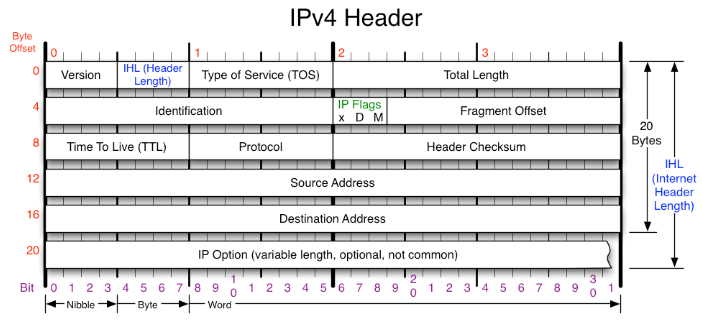
\includegraphics[width=\textwidth]{img/ipv4header.png}
	\caption{IPv4 Packet Header \cite{ipv6}}
	\label{fig:ipv4}
\end{figure}

\begin{itemize}
	\item Version - IP version number (set to 4 for IPv4)
	\item Internet Header Length (IHL) - Specifies the size of the header since a IPv4 header can be of varying length
	\item Type of Service (TOS) - As of RFC 2474 redefined to be differentiated services code point (DSCP) which is used by real time data streaming services like voice over IP (VoIP) and explicit congestion notification (ECN) which allows end-to-end notification of network congestion without dropping packets
	\item Total Length - Defines the entire packet size (header + data) in bytes. Min length is 20 bytes and max length is 65,535 bytes, although datagrams may be fragmented.
	\item Identification - Used for uniquely identifying the group of fragments of a single IP datagram
	\item X Flag - Reserved, must be zero
	\item DF Flag - If set, and fragmentation is required to route the packet, then the packet will be dropped. Usually occurs when packet destination doesn't have enough resources to handle incoming packet.
	\item MF Flag - If packet isn't fragmented, flag is clear. If packet is fragmented and datagram isn't the last fragment of the packet, the flag is set.
	\item Fragment Offset - Specifies the offset of a particular fragment relative to the beginning of the original unfragmented IP datagram
	\item Time To Live (TTL) - Limits the datagrams lifetime specified in seconds. In reality, this is actually the hop count which is decremented each time the datagram is routed. This helps to stop circular routing.
	\item Protocol - Defines the protocol used the data of the datagram
	\item Header Checksum - Used for to check for errors in the header. Router calculates checksum and compares to this value, discarding if they don't match.
	\item Source Address - Sender of the packet
	\item Destination Address - Receiver of the packet
	\item Options - specifies a number of options which are applicable for each datagram. As this project doesn't concern these it won't be discussed further.
\end{itemize}

\subsubsection{Packet Handling}
\label{subsec:handling}
Once the kernel of the given operating system has received data to transmit from a given application, the data is then placed into a packet with the correct header and these packets are placed on a IP stack (Figure~\ref{fig:buffer}). Through a few intermediate steps the packets arrive at the driver queue, also known as the transmission queue. This queue is implemented as a ring buffer, therefore has a maximum capacity before it starts to overwrite packets which are still to be transmitted. As long as the queue isn't empty, the network interface card (NIC) will take packets from the queue and place them on the transmission medium. A similar process occurs when receiving packets, but in the opposite direction. For each NIC, there is a receive and transmit queue which are independent of each other allow communication to be bidirectional, although this depends on the kernel and its handling of events associated with packets.

\begin{figure}[H]
	\centering
	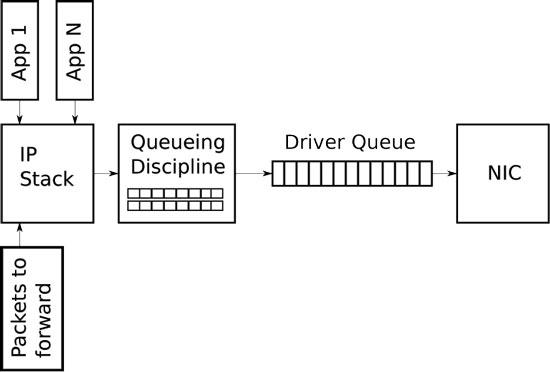
\includegraphics[width=\textwidth]{img/buffer.jpg}
	\caption{Linux packet handling \cite{buffer}}
	\label{fig:buffer}
\end{figure}


\subsubsection{Network Address Translator (NAT)}
As a routing device, a NAT is responsible for remapping an IP address to another by altering the IP datagram packet header. NAT's have become extremely important in modern networking systems due to IPv4 address exhaustion, allowing a single public IP address to map to multiple private IP addresses. This is particularly useful in large corporations where only a limited public network connection is required, meaning that all private IP addresses (usually associated with a single machine) are mapped to the same public IP address. A NAT will make use of multiple connection ports to identify which packets are for which private IP address and then re-assign the packet header so the internal routers can forward the packet correctly. As can be seen by Table~\ref{tab:ip} and Figure~\ref{fig:nat}, each internal address is mapped to via the port number associated with the external address. NAT's are generally implemented as part of a network firewall as they inspect the datagram packets for malicious data and sources.

\begin{table}[H]
	\centering
	\begin{tabular} { | c | c | }
		\hline
		\textbf{Private IP Address} & \textbf{Public IP Address} \\
		\hline
		10.0.0.1 & 14.1.23.5:62450 \\
		\hline
		10.0.0.2 & 14.1.23.5:62451 \\
		\hline
		10.0.0.3 & 14.1.23.5:62452 \\
		\hline
		10.0.0.4 & 14.1.23.5:62453 \\
		\hline
	\end{tabular}
	\caption{Example of public IP address and ports mapping to private IP address}
	\label{tab:ip}
\end{table}

\begin{figure}[H]
	\centering
	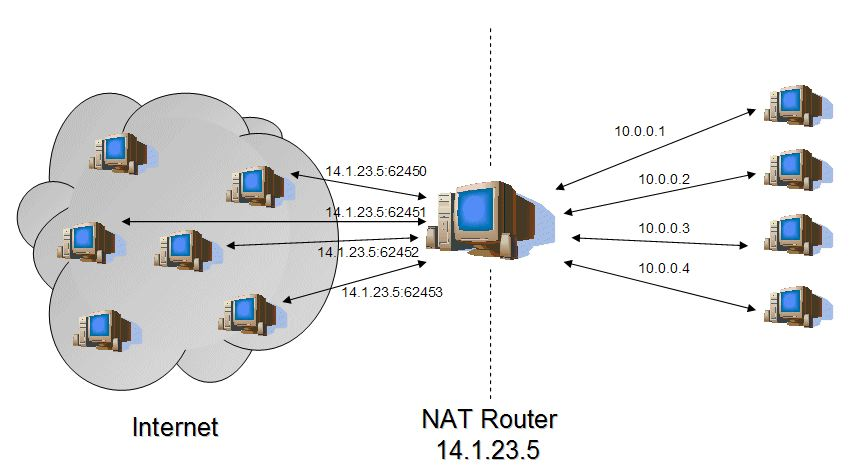
\includegraphics[width=\textwidth]{img/nat.jpg}
	\caption{NAT translating public IP addresses into private IP addresses \cite{nat-table}}
	\label{fig:nat}
\end{figure}

\subsubsection{Firewall}
Firewalls (Figure~\ref{fig:firewall}) are generally the major applications which sits between the public and private network of a system. They provide packet filtering which controls which packets can enter the private network via establishing a set of rules which packets have to adhere to. Filtering can be based on a number attributes of the packet such as the source and destination IP address and port and the destination service. Firewalls can also offer a number of other useful features such as NAT's or dynamic host configuration protocol (DCHP). As well as providing protection on a network level, application layer firewalls exist which stop certain applications from sending or receiving a packet. \\
\newline
Within this project, the term 'firewall' is used for a network layer firewall which filters packets dependent on the source IP address. Any changes in this will be mentioned within the relevant sections. \\

\begin{figure}[H]
	\centering
	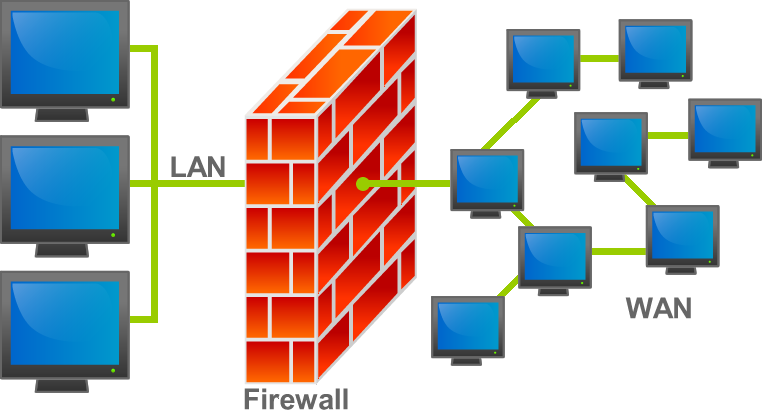
\includegraphics[width=0.7\textwidth]{img/firewall.png}
	\caption{Firewall intercepting packets as a security measure \cite{firewall}}
	\label{fig:firewall}
\end{figure}

\subsection{Java Features}
As the Java language and the JVM implementation is known by most, this section will focus on the more specific sections related to this project, instead of discussing the overall implementation.

\subsubsection{Java Virtual Machine (JVM)}
The Java Virtual Machine is an abstract computer that allows Java programs to run on any computer without dependant compilation. It provides an appealing coding language due to the vast support, frameworks and code optimisations available such as garbage collections and multithreading. Figure~\ref{fig:jvm} shows the basic JVM architecture with the relevant sections explained in the list below.

\begin{figure}[H]
	\centering
	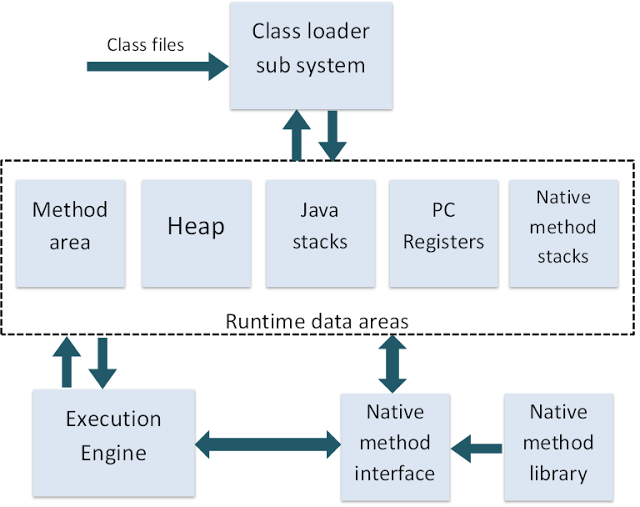
\includegraphics[width=\textwidth]{img/jvm.png}
	\caption{Java Virtual Machine interface \cite{jvm}}
	\label{fig:jvm}
\end{figure}

\begin{itemize}
	\item Class loader sub system - Loads .class files into memory, verifies byte code instructions and allocates memory required for the program
	\item Method area - stores class code and method code
	\item Heap - New objects are created on the heap
	\item Stack - Where the methods are executed and contains frames where each frame executes a separate method
	\item PC registers - Program counter registers store memory address of the instruction to be executed by the micro processor
	\item Native method stack - Where the native methods are executed.
	\item Native method interface - A program that connects the native method libraries with the JVM
	\item Native method library - holds the native libraries information
	\item Execution engine - Contains the interpreter and just in time compiler (JIT - converts byte code to machine code). JVM decides which parts to be interpreted and when to use JIT compiler.
\end{itemize}

Typically, any network communication from a Java application occurs via the JVM and through the operating system. This is because the JVM is still technically an application running on top of the OS and therefore doesn't have any superuser access rights. Any network operation results in a kernel system call, which is then put into a priority queue in order to be executed. This is one of the main reasons why network calls through the JVM and kernel can be seen as 'slow', in relative speeds compared to network line rate speeds.

\subsubsection{Java Native Interface (JNI)}
Provided by the Java Software Development Kit (SDK), the JNI is a native programming interface that lets Java applications use libraries written in other languages. The JNI also includes the invocation API which allows a JVM to be embedded into native applications. This project and therefore this overview will only focus on Java code using C libraries via the JNI on a linux based system\\
\newline
In order to call native libraries from Java applications a number of steps have to be undertaken as shown below, which are described in more detail later:
\begin{enumerate}
	\item Java code - load the shared library, declare the native method to be called and call the method
	\item Compile Java code - compile the Java code into bytecode
	\item Create C header file - the C header file will declare the native method signature and is created automatically via a terminal call
	\item Write C code - write the corresponding C source file
	\item Create shared library - create a shared library file (.so) from C code
	\item Run Java program - run the Java program which calls the native code
\end{enumerate}

\begin{lstlisting}[language=Java, caption={Basic Java class showing native method declaration and calling with shared library loading}, label=lst:java]
public class Hello {
    public native void sayHi(String who, int times);

    static { System.loadLibrary("Hello"); }

    public static void main(String[] args) {
        Hello hello = new Hello();
        
        hello.sayHi(args[0], Integer.parseInt(args[1]));
    }
}
\end{lstlisting}

Code~\ref{lst:java} shows a simple Java program which uses some native C code from a shared library. Line 4 indicates which shared library to load into the application, which is by default lib*.so where * indicates the name of the C file. Line 2 is the native method declaration which specifies the name of the method and the parameters which will be passed to the corresponding C method. Line 9 is where this native method is called.

\begin{lstlisting}[language=sh, caption={Compiling basic Java program}, label=lst:javacomp]
$ javac Hello.java
\end{lstlisting}

Code~\ref{lst:javacomp}, run from a terminal, compiles the Java class and create a class file which can be executed.

\begin{lstlisting}[language=sh, caption={Generating C header file}, label=lst:gen]
$ javah -jni Hello.java
\end{lstlisting}

In order to generate the C header file the command 'javah' (Code~\ref{lst:gen}) is used with the flag 'jni' which tells Java that a header file is required which is for use with the JNI. It will then produce method signatures which correspond to the native method declared within Hello.java. The auto generated C header file is shown in Code~\ref{lst:auto}.

\begin{lstlisting}[language=C, caption={Auto-generated C header file}, label=lst:auto]
/* DO NOT EDIT THIS FILE - it is machine generated */
#include <jni.h>
/* Header for class Hello */

#ifndef _Included_Hello
#define _Included_Hello
#ifdef __cplusplus
extern "C" {
#endif
/*
 * Class:     Hello
 * Method:    sayHi
 * Signature: (Ljava/lang/String;I)V
 */
JNIEXPORT void JNICALL Java_Hello_sayHi
  (JNIEnv *, jobject, jstring, jint);

#ifdef __cplusplus
}
#endif
#endif
\end{lstlisting}

\begin{lstlisting}[language=C, caption={C source file corresponding to auto-generated header file}, label=lst:source]
#include <stdio.h>
#include "Hello.h"

JNIEXPORT void JNICALL Java_Hello_sayHi
(JNIEnv *env, jobject obj, jstring who, jint times) {
    jint i;
    jboolean iscopy;
    const char *name;
    name = (*env)->GetStringUTFChars(env, who, &iscopy);
    for (i = 0; i < times; i++) {
        printf("Hello %s\n", name);
    }
}
\end{lstlisting}

The C source file implementation is in Code~\ref{lst:source}. Line 9 is the interesting line, where the code is retrieving the string stored at pointer 'who' from the Java environment and copying it into the pointer 'name' for use later on.

\begin{lstlisting}[language=sh, caption={Terminal commands to generate shared library file (.so)}, label=lst:shared]
$ cc -c -I/System/Library/Frameworks/JavaVM.framework/Headers Hello.c
$ cc -dynamiclib -o libhello.so Hello.o -framework JavaVM
\end{lstlisting}

The 2 commands in Code~\ref{lst:shared} will first compile the C source code into an object file (.o), requiring a pointer to the jni.h file provided with the Java framework. The second line then generates the required shared object file (.so) which the Java application looks for.

\begin{lstlisting}[language=sh, caption={Output from running Java application calling native C methods}, label=lst:output]
$ java Hello Packet-Processing 5
Packet-Processing
Packet-Processing
Packet-Processing
Packet-Processing
Packet-Processing
\end{lstlisting}

Running the Java application with the required parameters will output the above in Code~\ref{lst:output}. \\
\newline
As can be seen in the example code (Code~\ref{lst:source}), there are 2 extra parameters in the method signature that weren't defined within the Java native method signature (Code~\ref{lst:java}). The 'env' pointer is a structure that contains the interface to the JVM, therefore providing numerous functions required to interact with the JVM and the Java objects. Examples include converting native arrays to Java arrays and throwing exceptions, allowing standard Java operations to be executed within the native C libraries via this interface. \\
\newline
The 'obj' argument refers to the Java object which the native method had been declared within. \\
\newline
Although the JNI provides a very useful interface to interact with native library code, there are a number of issues that users should be wary of before progressing:
\begin{itemize}
	\item The Java application that relies on the JNI loses its portability with the JVM as it relies on natively compiled code.
	\item Errors within the native code can potentially crash the JVM, with certain errors been very difficult to reproduce and debug.
	\item Anything instantiated with the native code won't be collected by the garbage collector with the JVM, so freeing memory should be a concern.
	\item If using the JNI on large scale, converting between Java objects and C structs can be difficult
\end{itemize}

\subsubsection{Current Java Networking Methods}
For high performance computing in Java, a number of existing programming options are available in order for applications to communicate over a network. These can be classified as: (1) Java sockets; and (2) Remote Method Invocation (RMI); (3) shared memory programming. As will be discussed, none of these are capable of truly high performance networking, especially at line rate speeds.

\paragraph{Java Sockets}\mbox{}\\ %subsubsubsection
\label{subsec:sockets}
Java sockets are the standard low level communication for applications as most networking protocols have socket implementations. They allow for streams of data to be sent between applications as a socket is one end point for a 2 way communication link, meaning that data can be read from and written to a socket in order to transfer data. Even though sockets are a viable option for networking, both of the Java socket implementations (IO sockets \& NIO (new I/O) sockets) are inefficient over high speed networks \cite{sockets} and therefore lack the performance that is required. As discussed previously, the poor performance is due to the JVM interacting with network cards via the OS kernel.

\paragraph{Remote Method Invocation (RMI)}\mbox{}\\ %subsubsubsection
Remote Method Invocation (RMI) is a protocol developed by Java which allows an object running in a JVM to invoke methods on another object running on a different JVM. Although this method provides a relatively easy interface for which JVM's can communicate, its major drawback relates to the speed. Since RMI uses Java sockets as its basic level communication method, it faces the same performance issues as mentioned in section~\ref{subsec:sockets}.

\paragraph{Shared Memory Programming}\mbox{}\\ %subsubsubsection
Shared memory programming provides high performance JVM interaction due to Java's multithread and parallel programming support. This allows different JVM's to communicate via objects within memory which is shared between the JVM's. However, this technique requires the JVM's to be on the same shared memory system, which is a major drawback for distributed systems as scalability options decrease. \\

Even though these 3 techniques allow for communication between JVM's, the major issue is that incoming packets are still handled by the kernel and then passed onto the corresponding JVM. This means that packets are destined for certain applications, meaning that generic packets can't be intercepted and checked, which is a requirement for generic middlebox software. There is also the issue that all packets are processed via the kernel, which is a major speed reducer which limits the line rate.

\subsection{jVerbs}
Ultra-low latency for Java applications has been partially solved by the jVerbs \cite{jverbs} framework. Using remote direct memory access (RDMA), jVerbs provides an interface for which Java applications can communicate, mainly useful within large scale data centre applications. \\
\newline
RDMA is a technology that allows computers within a network to transfer data between each other via direct memory operations, without involving the processor, cache or operating system of either communicating computer. RDMA implements a transport protocol directly within the network interface card (NIC), allowing for zero copy networking, which allows a computer to read from another computer and write to its own direct main memory without intermediate copies. High throughput and performance is a feature of RDMA due to the lack of kernel involvement, but the major downside is that it requires specific hardware which supports the RDMA protocol, while also requiring the need for specific computer connections set up by sockets. \\
\newline
As jVerbs takes advantage of mapping the network device directly into the JVM, bypassing both the JVM and operating system (Figure~\ref{fig:jverb}), it can significantly reduce the latency. In order to have low level interaction with the NIC, jVerbs has a very thin layer of JNI calls which can increase the overhead slightly. However, jVerbs is flawed, mainly because it requires specific hardware to run on, firstly limited by the RDMA protocol reliant hardware and further by the required RDMA wrappers which are implemented by the creators. Also, it can only be used for specific computer to computer connection and not generally packet inspection. 

\begin{figure}[H]
	\centering
	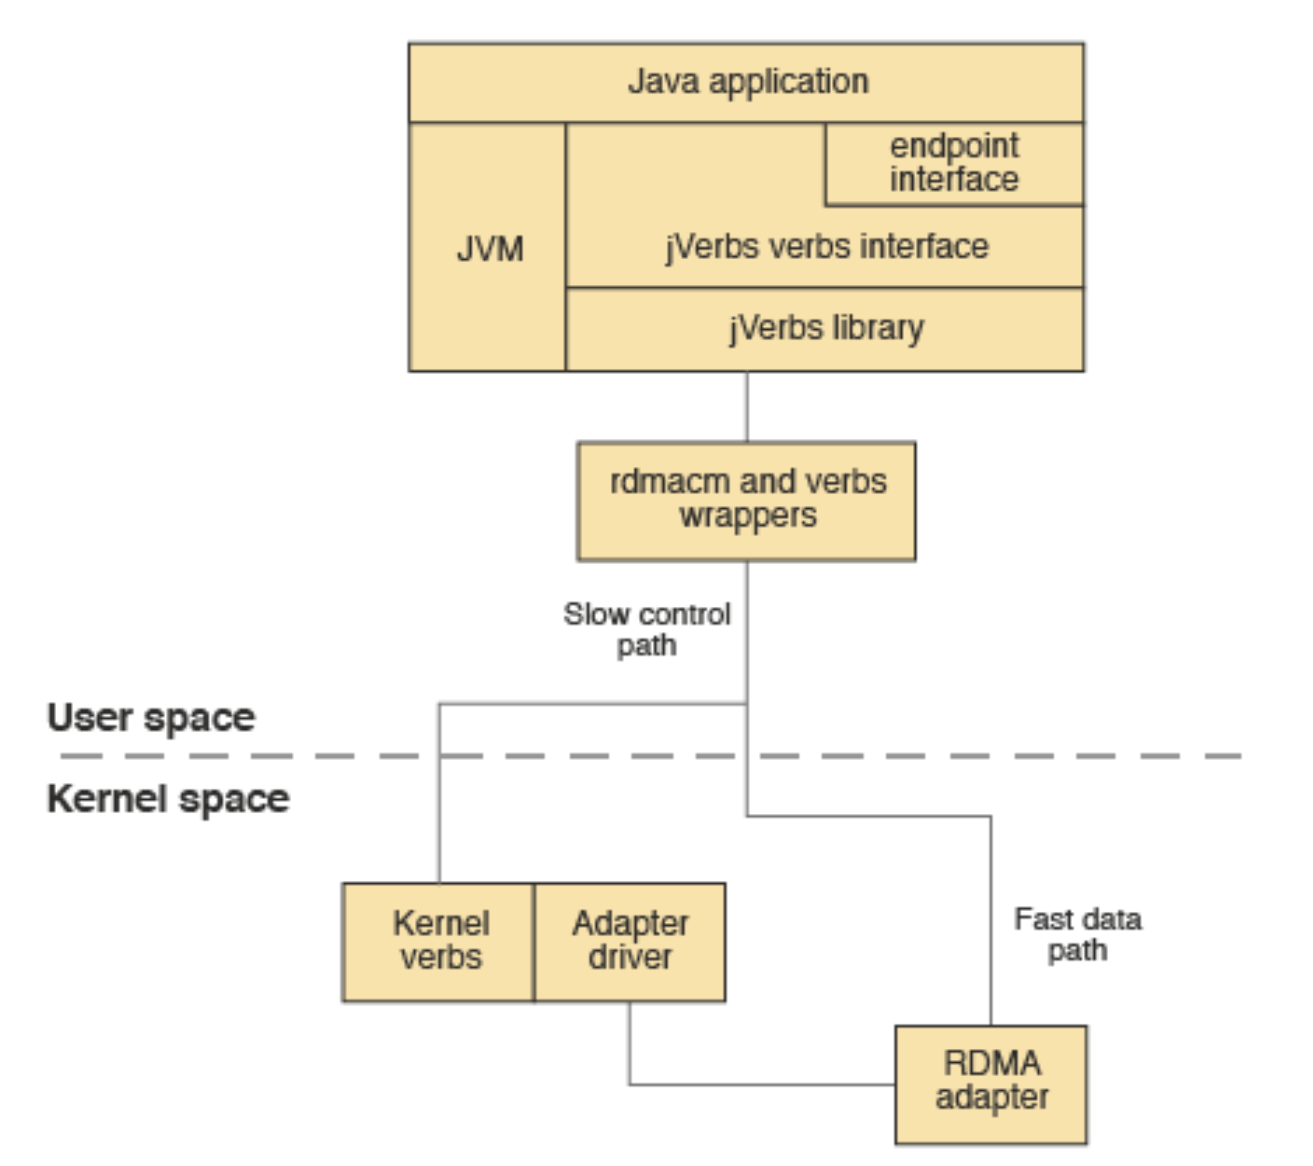
\includegraphics[width=\textwidth]{img/jverbs.png}
	\caption{jVerbs architecture - shows how the framework bypasses the kernel and JVM \cite{ibm_jverbs}}
	\label{fig:jverb}
\end{figure}

jVerbs provides a useful example framework which re-emphasises that packet processing in Java is very possible with low latency, while assisting in certain implementation and design choices which can be analysed in more detail. 

\subsection{Native I/O API's}
Currently available native networking API's are capable of reading and writing packets to the NIC transmission and receive queues at line rate. This is due to a number of techniques which tend to alter the kernels understand of the underlying NIC, therefore requiring specialist hardware and software to use such tools. DPDK (Section~\ref{subsec:dpdk}) is one of the tools that is open source and publicly available for use.

\subsubsection{Data Plane Development Kit (DPDK)}
\label{subsec:dpdk}
Data Plane Development Kit (DPDK) \cite{dpdk} is a set of libraries and drivers which enabaled fast packet processing with certain system set ups. Since DPDK is developed by Intel, it only supports Intel x86 CPU's and certain network interface controllers. DPDK overwrites the NIC's drivers meaning that the operating system doesn't recognise the network cards and can't interact with them. It installs its own drivers allowing it to interact with certain memory locations without permission from the kernel or even involving it in any way. \\
\newline
DPDK makes use of an environment abstraction layer (EAL) which hides the environmental specifics and provides a standard interface which any application can interact with. Due to this, if the system changes in any way, the DPDK library needs to be re-compiled with other features been re-enabled in order to allow applications to run correctly again. \\
\newline
DPDK also makes use of 'Hugepages', which are memory locations of 2mb size rather than the standard 4kb size, while also forcing the user to reserve these 'Hugepage' locations at initial boot. It uses these memory locations to store packets in the corresponding ring buffer as mentioned in Section~\ref{subsec:handling}. \\
\newline
In order to use the DPDK libraries for the intended purpose, data packets have to be written into the correct buffer location so they are inserted onto the network. I similar approach is used when receiving packets on the incoming buffer ring, but instead of the system using interrupts to acknowledge the arrival of a new packet, which is performance costly, it constantly polls the buffer space to check for new packets. DPDK also allows for multiple queues per NIC and can handle multiple NIC's per system, therefore scalability is a major bonus of the libraries. \\
\newline
DPDK is very well documented on a number of levels. Firstly there is a online API which gives in depth details about what the methods, constants and structs do. There are a number of well written guides which give step-by-step details of how to install, set-up and use DPDK on various platforms and finally, there are many sample programs included with the build which give understanding of how the overall library works.


\end{document}